% Provenance (never printed): cycle 3 "Matiere, mouvement, energie,
% information" and "La planete Terre" (meteorological phenomena, the water in
% the air, measuring the weather); see sources/book1/PROVENANCE.md.
% Book 1, grade 4, chapter 1.
\chapter{السحب والمطر والثلج}\label{ch:g4:clouds-rain-snow}

بعد ظهر يوم صيفي حار. عند الغداء كانت السماء زرقاء، فيها بضع \omterm{def:g4:clouds-rain-snow:cloud}{سحب} بيضاء
صغيرة كأنها كرات من القطن. وعند الساعة الثالثة كبرت إحداها. إنها تنتفخ
نحو الأعلى، أعلى فأعلى، كقرنبيط أبيض قائم على قاعدة رمادية مسطحة. ثم
تنبسط قمتها، وتسودّ قاعدتها. تهب نفحة من ريح باردة، وتسقط أولى القطرات
الكبيرة، ويهطل \omterm{def:g4:clouds-rain-snow:precipitation}{المطر} غزيرًا عشرين دقيقة. ثم تبتعد \omterm{def:g4:clouds-rain-snow:cloud}{السحابة}، وتعود الشمس،
ويتصاعد البخار من الأرصفة المبللة.

من أين جاءت تلك \omterm{def:g4:clouds-rain-snow:cloud}{السحابة}؟ ومم تتكون؟ وكم من \omterm{def:g4:clouds-rain-snow:precipitation}{المطر} سقط في تلك الدقائق
العشرين؟

\begin{recall}
\omterm{def:g1:watching-the-weather:weather}{الطقس} هو حال الهواء في مكان ولحظة معيّنين: مشمس، غائم، ماطر، مثلج، عاصف،
ضبابي؛ ونسجله في \omterm{def:g1:watching-the-weather:weather-chart}{جدول الطقس} (\cref{ch:g1:watching-the-weather}). والماء
يصعد من \omterm{def:g2:water-on-earth:ocean}{البحر} \omterm{def:g1:landscapes-around-us:water}{والبحيرات} والأرض إلى الهواء، ثم يعود فينزل مطرًا
(\cref{ch:g2:water-on-earth}). وكتب الفيزياء تحكي كيف يتبخر الماء (من
سائل إلى غاز لا يُرى)، وكيف يتكاثف (من غاز إلى قطيرات سائلة صغيرة جدًا)،
وكيف يتجمد (من سائل إلى جليد)، وكيف يقيس مقياس الحرارة درجة الحرارة
بالدرجات المئوية.
\end{recall}

\section{ما السحابة؟}

الهواء من حولنا يحمل دائمًا شيئًا من الماء، غازًا لا يُرى: بخار الماء.
وحين يصعد الهواء يبرد. وحين يبرد بما يكفي، يتكاثف جزء من بخار مائه قطيراتٍ
صغيرة جدًا حتى إن أخف نسمة تبقيها معلقة. وبلايين من هذه القطيرات، بعضها
بجانب بعض، تصنع \omterm{def:g4:clouds-rain-snow:cloud}{سحابة} نراها. وفي الأعالي، حيث الهواء شديد البرودة، تتجمد
القطيرات، فتتكون \omterm{def:g4:clouds-rain-snow:cloud}{السحابة} من قطع صغيرة جدًا من الجليد.

\begin{definition}[السحابة والضباب]\label{def:g4:clouds-rain-snow:cloud}
\emph{السحابة}\index{سحابة} عدد كبير جدًا من قطيرات الماء الصغيرة جدًا،
أو من قطع الجليد الصغيرة جدًا، معلقة معًا في الهواء. و\emph{الضباب}\index{ضباب}
سحابة تلامس الأرض.
\end{definition}

\begin{example}[أنفاسك في صباح بارد]\label{ex:g4:clouds-rain-snow:breath}
في صباح بارد، تصنع أنفاسك \omterm{def:g4:clouds-rain-snow:cloud}{سحابة} بيضاء صغيرة أمام فمك. فالهواء الذي تزفره
دافئ ويحمل بخار الماء. والهواء البارد يبرّده فورًا، فيتكاثف البخار قطيراتٍ
صغيرة جدًا --- وتظهر \omterm{def:g4:clouds-rain-snow:cloud}{سحابة} مصغرة، ثم تختفي حين تتبخر القطيرات من
جديد.
\end{example}

\omterm{def:g4:clouds-rain-snow:cloud}{السحابة} بيضاء لأن قطيراتها تشتت ضوء الشمس في كل الاتجاهات. وحين تكون
كثيفة جدًا لا يصل إلى قاعدتها إلا قليل من الضوء، فتبدو من الأسفل رمادية
أو شبه سوداء: وتلك علامة \omterm{def:g4:clouds-rain-snow:cloud}{سحابة} ثقيلة مليئة
بالماء.

\section{فصائل السحب}

\omterm{def:g4:clouds-rain-snow:cloud}{للسحب} أشكال كثيرة، ومراقبو \omterm{def:g1:watching-the-weather:weather}{الطقس} في العالم كله يصنّفونها بالطريقة نفسها،
بحسب شكلها وبحسب الارتفاع الذي تطفو عنده.

\begin{definition}[فصائل السحب]\label{def:g4:clouds-rain-snow:cloud-families}
فصائل \omterm{def:g4:clouds-rain-snow:cloud}{السحب} الأربع التي يجب أن تعرفها هي:
\begin{itemize}
  \item \emph{الركام}\index{ركام}: \omterm{def:g4:clouds-rain-snow:cloud}{سحب} متراكمة، بيضاء منتفخة، قاعدتها
        مسطحة، كأنها كرات من القطن؛
  \item \emph{الطبقي}\index{طبقي}: \omterm{def:g4:clouds-rain-snow:cloud}{سحب} طبقية، غطاء رمادي مسطح يغطي
        السماء كلها، منخفض؛
  \item \emph{السمحاق}\index{سمحاق}: \omterm{def:g4:clouds-rain-snow:cloud}{سحب} خيطية، خيوط أو خصلات بيضاء رقيقة،
        عالية جدًا، مكونة من الجليد؛
  \item \emph{الركام المزني}\index{ركام مزني}: \omterm{def:g4:clouds-rain-snow:cloud}{سحابة} العاصفة، برج ضخم
        يرتفع من قاعدة داكنة منخفضة إلى ارتفاع كبير جدًا، وكثيرًا ما تنبسط
        قمته مسطحة.
\end{itemize}
\end{definition}

وهذه أسماء تصف الشكل، وهي ترجمة لأسماء لاتينية: \emph{\omterm{def:g4:clouds-rain-snow:cloud-families}{الركام}} الكومة،
و\emph{\omterm{def:g4:clouds-rain-snow:cloud-families}{الطبقي}} من الطبقة، و\emph{\omterm{def:g4:clouds-rain-snow:cloud-families}{السمحاق}} خصلة الشعر، و\emph{المزن} \omterm{def:g4:clouds-rain-snow:cloud}{سحب} \omterm{def:g4:clouds-rain-snow:precipitation}{المطر}.

\begin{omfigure}
\begin{minipage}[b]{0.49\linewidth}\centering
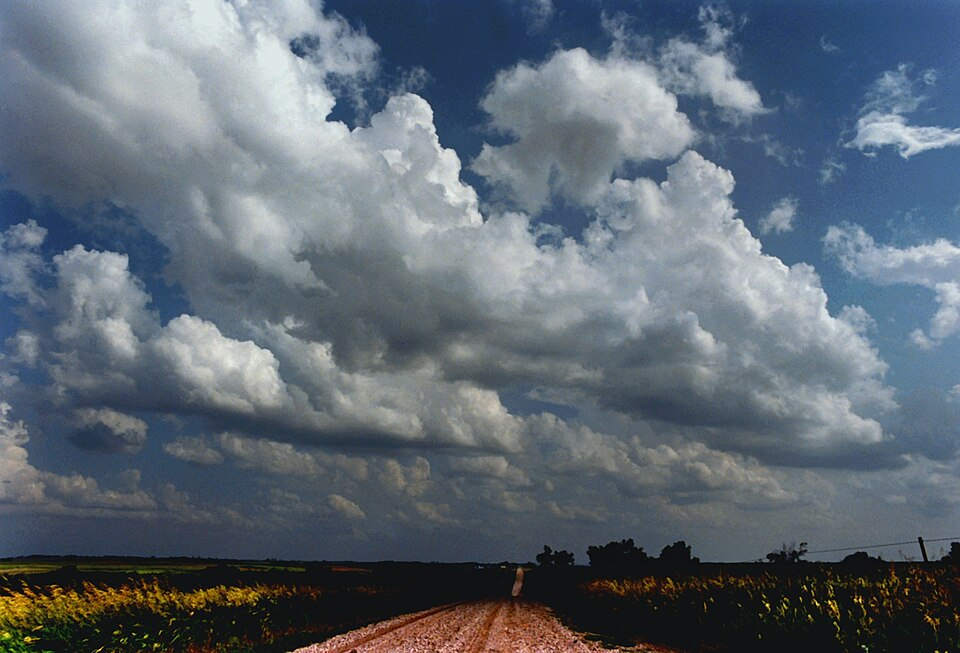
\includegraphics[width=\linewidth]{images/book1/g4-cumulus.jpg}

{\small \omterm{def:g4:clouds-rain-snow:cloud-families}{الركام}: \omterm{def:g4:clouds-rain-snow:cloud}{سحب} متراكمة قواعدها مسطحة.}
\end{minipage}\hfill
\begin{minipage}[b]{0.49\linewidth}\centering
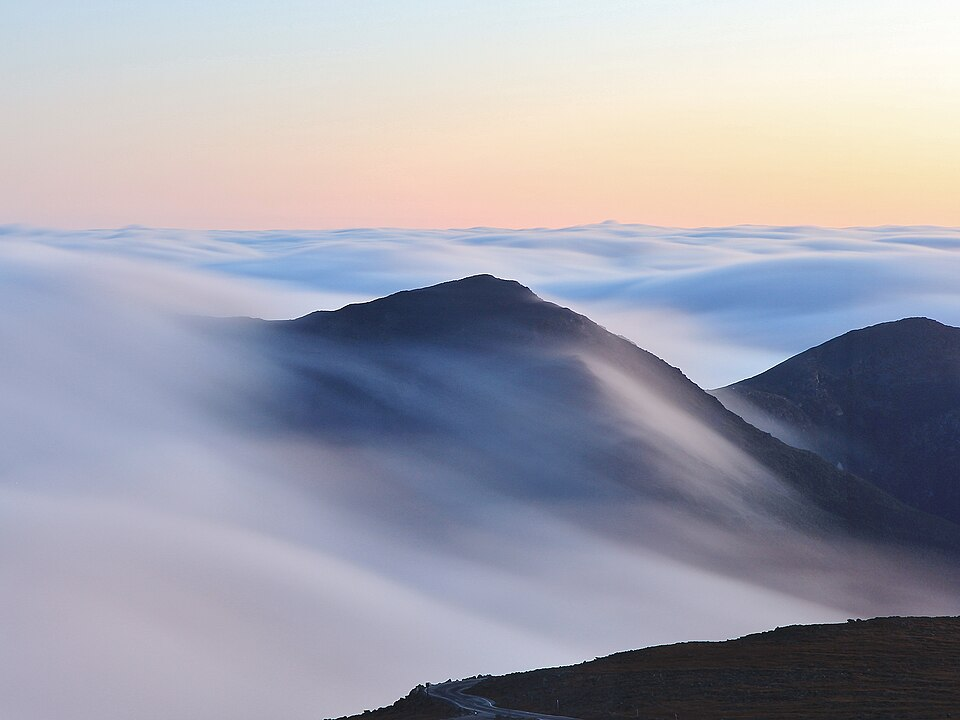
\includegraphics[width=\linewidth]{images/book1/g4-stratus.jpg}

{\small \omterm{def:g4:clouds-rain-snow:cloud-families}{الطبقي}: طبقة مسطحة، تُرى هنا من الأعلى، من \omterm{def:g1:landscapes-around-us:landform}{جبل}.}
\end{minipage}

\medskip
\begin{minipage}[b]{0.49\linewidth}\centering
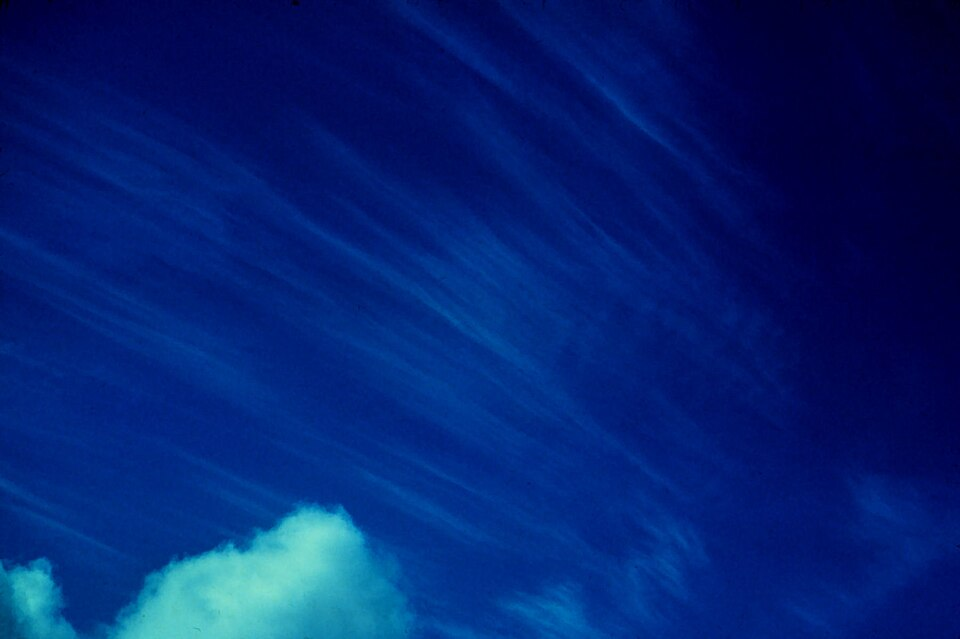
\includegraphics[width=\linewidth]{images/book1/g4-cirrus.jpg}

{\small \omterm{def:g4:clouds-rain-snow:cloud-families}{السمحاق}: خيوط رقيقة من الجليد، عالية جدًا (وتحتها \omterm{def:g4:clouds-rain-snow:cloud-families}{ركام} صغير).}
\end{minipage}\hfill
\begin{minipage}[b]{0.49\linewidth}\centering
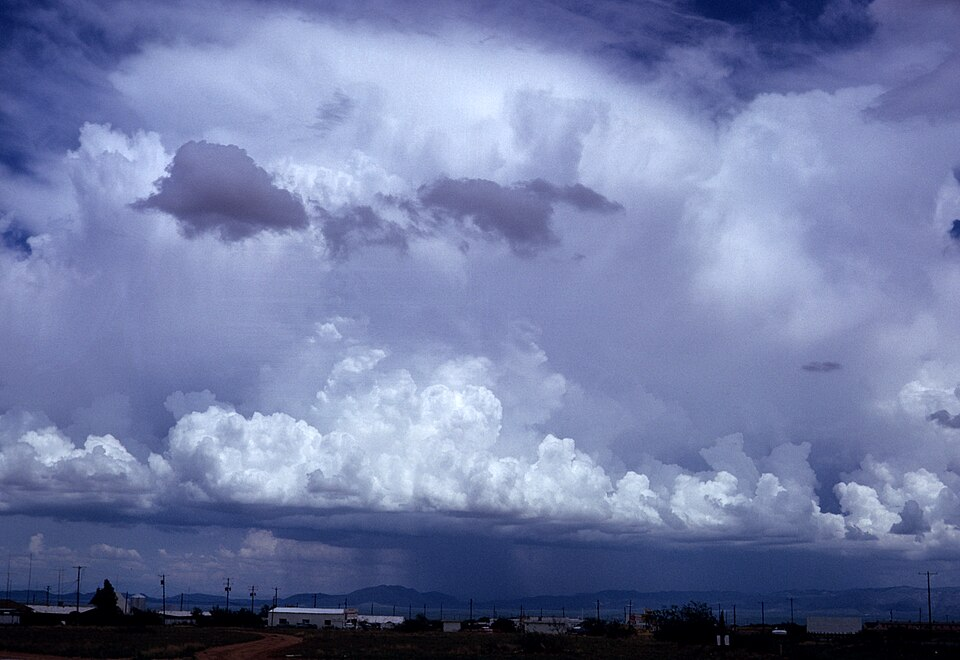
\includegraphics[width=\linewidth]{images/book1/g4-cumulonimbus.jpg}

{\small \omterm{def:g4:clouds-rain-snow:cloud-families}{ركام مزني}: برج من السحاب؛ \omterm{def:g4:clouds-rain-snow:precipitation}{والمطر} يسقط من قاعدته الداكنة.}
\end{minipage}

\smallskip
{\small الصور: مكتبة صور NOAA (ملك عام): س. كورفيدي
(\omterm{def:g4:clouds-rain-snow:cloud-families}{الركام})، ر. ف. كريسغ (\omterm{def:g4:clouds-rain-snow:cloud-families}{السمحاق})، مجموعة ب. هوك (\omterm{def:g4:clouds-rain-snow:cloud-families}{الركام المزني}).}
% ledger: noaa:photos-g4
\label{fig:g4:clouds-rain-snow:photos}
\end{omfigure}

على أي ارتفاع تطفو \omterm{def:g4:clouds-rain-snow:cloud}{السحب}؟ ذلك يتوقف على الفصيلة. \omterm{def:g4:clouds-rain-snow:cloud}{فالسحب} المنخفضة، مثل
\omterm{def:g4:clouds-rain-snow:cloud-families}{الطبقي} وقاعدة \omterm{def:g4:clouds-rain-snow:cloud-families}{الركام}، تطفو من فوق الأرض مباشرة حتى نحو 2 كيلومتر. أما
\omterm{def:g4:clouds-rain-snow:cloud-families}{السمحاق} فيطفو عاليًا جدًا، بين نحو 5 و13
كيلومترًا خارج المناطق المدارية والقطبية --- وكثيرًا ما يكون أعلى من أعلى
\omterm{def:g1:landscapes-around-us:landform}{جبل} على الأرض.
ويمتد \omterm{def:g4:clouds-rain-snow:cloud-families}{الركام المزني} من قاعدة منخفضة حتى أعلى مستويات
\omterm{def:g4:clouds-rain-snow:cloud}{السحب}.
% ledger: wmo:cloud-levels, wmo:cumulonimbus

\begin{omfigure}
\begin{tikzpicture}[x=1cm, y=0.5cm, font=\small]
  % height scale
  \draw[black!60] (0,0) -- (0,14);
  \foreach \h in {0,2,...,14} {
    \draw[black!60] (-0.1,\h) -- (0,\h);
    \node[anchor=east, font=\scriptsize] at (-0.12,\h) {\h\,km};
  }
  \node[anchor=south, font=\scriptsize, align=center] at (0,14.2) {الارتفاع};
  % ground and a mountain for comparison
  \fill[green!35!black!50] (0.2,0) -- (11.4,0) -- (11.4,-0.4) -- (0.2,-0.4) -- cycle;
  \fill[black!35] (8.6,0) -- (9.9,8.8) -- (10.2,8.4) -- (11.2,0) -- cycle;
  \fill[white, draw=black!45, line width=0.3pt] (9.65,7.2) -- (9.9,8.8) -- (10.2,8.4) -- (10.4,7.0) -- (10.1,7.4) -- (9.9,7.0) -- cycle;
  \node[font=\scriptsize, align=center] at (9.9,10.2) {أعلى\\جبل};
  % levels
  \fill[blue!6] (0.2,0.15) rectangle (8.3,2);
  \fill[blue!10] (0.2,5) rectangle (8.3,13);
  \node[anchor=west, font=\scriptsize, text=blue!50!black] at (0.3,1.65) {سحب منخفضة};
  \node[anchor=west, font=\scriptsize, text=blue!50!black] at (0.3,12.6) {سحب عالية};
  % stratus: a flat grey layer
  \fill[black!25, rounded corners=2pt] (0.6,0.6) rectangle (2.6,1.3);
  \node[font=\scriptsize] at (1.6,-1.1) {الطبقي};
  % cumulus
  \pic[scale=0.7, transform shape] at (4.0,0.9) {puffycloud};
  \node[font=\scriptsize] at (4.0,-1.1) {الركام};
  % cirrus: wisps
  \foreach \y in {9.4,10.0,10.6} {
    \draw[black!50, line width=0.6pt] (0.8,\y) .. controls (1.4,\y+0.5) and (2.0,\y+0.1) .. (2.6,\y+0.6);
  }
  \node[font=\scriptsize] at (1.7,8.5) {السمحاق};
  % cumulonimbus: tower with an anvil
  \fill[black!15, draw=black!45, line width=0.4pt]
    (5.4,1.0) .. controls (5.2,4) and (5.6,8) .. (5.9,11.2)
    .. controls (5.0,11.6) and (4.6,12.0) .. (4.8,12.3)
    -- (8.1,12.3) .. controls (8.2,12.0) and (7.8,11.6) .. (7.0,11.2)
    .. controls (7.3,8) and (7.6,4) .. (7.4,1.0) -- cycle;
  \fill[black!45] (5.4,1.0) rectangle (7.4,1.4);
  \foreach \x in {5.7,6.1,6.5,6.9,7.2}
    \draw[omWxRain, line width=0.6pt] (\x,0.95) -- (\x-0.15,0.15);
  \node[font=\scriptsize] at (6.4,-1.1) {الركام المزني};
\end{tikzpicture}

{\small الارتفاع الذي تطفو عنده فصائل \omterm{def:g4:clouds-rain-snow:cloud}{السحب} الأربع (الارتفاعات بالكيلومتر، في
مناطق ليست مدارية ولا قطبية). \omterm{def:g4:clouds-rain-snow:cloud-families}{الطبقي} وقاعدة \omterm{def:g4:clouds-rain-snow:cloud-families}{الركام} منخفضان؛ \omterm{def:g4:clouds-rain-snow:cloud-families}{والسمحاق} كثيرًا
ما يكون أعلى من أعلى \omterm{def:g1:landscapes-around-us:landform}{جبل}. ويمتد \omterm{def:g4:clouds-rain-snow:cloud-families}{الركام المزني} من قاعدة منخفضة حتى أعلى
مستويات \omterm{def:g4:clouds-rain-snow:cloud}{السحب}. الارتفاعات بحسب أطلس \omterm{def:g4:clouds-rain-snow:cloud}{السحب} للمنظمة العالمية للأرصاد
الجوية.}
\label{fig:g4:clouds-rain-snow:heights}
% ledger: wmo:cloud-levels, tht:everest
\end{omfigure}

\begin{method}[تسمية السحابة]\label{met:g4:clouds-rain-snow:naming}
انظر إلى السماء واطرح ثلاثة أسئلة:
\begin{enumerate}
  \item هل هي كومة قاعدتها مسطحة؟ إذن هي \omterm{def:g4:clouds-rain-snow:cloud-families}{ركام} --- وإن ارتفعت برجًا داكنًا
        ضخمًا، فهي \omterm{def:g4:clouds-rain-snow:cloud-families}{ركام مزني}.
  \item هل هي غطاء مسطح منتظم يحجب السماء كلها؟ إذن هي
        \omterm{def:g4:clouds-rain-snow:cloud-families}{طبقي}.
  \item هل تتكون من خيوط بيضاء رقيقة، عالية جدًا؟ إذن هي \omterm{def:g4:clouds-rain-snow:cloud-families}{سمحاق}.
\end{enumerate}
\end{method}

\begin{remark}[السحب تخبرنا بالطقس]\label{rem:g4:clouds-rain-snow:tell}
\omterm{def:g4:clouds-rain-snow:cloud-families}{الركام} الصغير في سماء زرقاء يعني طقسًا صحوًا. \omterm{def:g4:clouds-rain-snow:cloud-families}{والطبقي} الرمادي يأتي بيوم
كئيب، وأحيانًا برذاذ. \omterm{def:g4:clouds-rain-snow:cloud-families}{والركام المزني} يأتي بزخة قصيرة غزيرة، كثيرًا ما يرافقها
رعد وبرق وهبات ريح --- وأحيانًا \omterm{def:g4:clouds-rain-snow:precipitation}{برد}. أما \omterm{def:g4:clouds-rain-snow:cloud-families}{السمحاق} فلا يأتي \omterm{def:g4:clouds-rain-snow:precipitation}{بالمطر}، لكنه حين
ينتشر ويزداد كثافة كثيرًا ما يأتي \omterm{def:g4:clouds-rain-snow:precipitation}{المطر} بعده
بيوم.
\end{remark}

\section{المطر والثلج والبرد}

داخل \omterm{def:g4:clouds-rain-snow:cloud}{السحابة} تصطدم القطيرات الصغيرة جدًا بعضها ببعض فتتحد، أو تنمو بلورات
الجليد على حساب القطيرات. فإذا كبرت قطرة \omterm{def:g4:clouds-rain-snow:cloud}{السحابة}، أو البلورة، وثقلت بما
يكفي، لم تعد تستطيع أن تطفو: فتسقط.

\begin{definition}[الهطول]\label{def:g4:clouds-rain-snow:precipitation}
\emph{الهطول}\index{هطول} ماء يسقط من \omterm{def:g4:clouds-rain-snow:cloud}{سحابة} إلى الأرض: \emph{المطر}\index{مطر}
(قطرات من الماء السائل)، أو
\emph{الثلج}\index{ثلج} (ندف من بلورات جليد ملتصقة معًا)، أو
\emph{البرد}\index{برد} (كرات من الجليد تسمى حبات البرد، تسقط من
\omterm{def:g4:clouds-rain-snow:cloud}{سحب} العواصف).
\end{definition}

سقوط \omterm{def:g4:clouds-rain-snow:precipitation}{المطر} أو \omterm{def:g4:clouds-rain-snow:precipitation}{الثلج} يتوقف على درجة حرارة الهواء الذي يعبره \omterm{def:g4:clouds-rain-snow:precipitation}{الهطول}. فندف
\omterm{def:g4:clouds-rain-snow:precipitation}{الثلج} تتكون عاليًا في \omterm{def:g4:clouds-rain-snow:cloud}{السحابة} الباردة. فإذا كان الهواء تحتها فوق
\SI{0}{\celsius} مدة كافية، ذابت في طريقها إلى الأسفل ووصلت إلينا مطرًا. وإذا كان
الهواء متجمدًا طوال الطريق إلى الأرض، وصلت
ثلجًا.

\begin{omfigure}

\includegraphics[width=0.55\linewidth]{images/book1/ai/g4-snowflakes.jpg}

{\small أطفال يلتقطون ندف \omterm{def:g4:clouds-rain-snow:precipitation}{الثلج} على قفاز داكن: كل ندفة مكونة من
بلورات جليد.}
\end{omfigure}

لا يسقط \omterm{def:g4:clouds-rain-snow:precipitation}{البرد} إلا من \omterm{def:g4:clouds-rain-snow:cloud-families}{الركام المزني}. ففي داخل البرج ترفع رياح صاعدة قوية
حبيبات الجليد وتنزلها مرات عدة؛ وكل رحلة تضيف طبقة جديدة من الجليد، كطبقات
البصلة، حتى تصير حبة \omterm{def:g4:clouds-rain-snow:precipitation}{البرد} أثقل من أن تحملها
الريح.

\begin{omfigure}
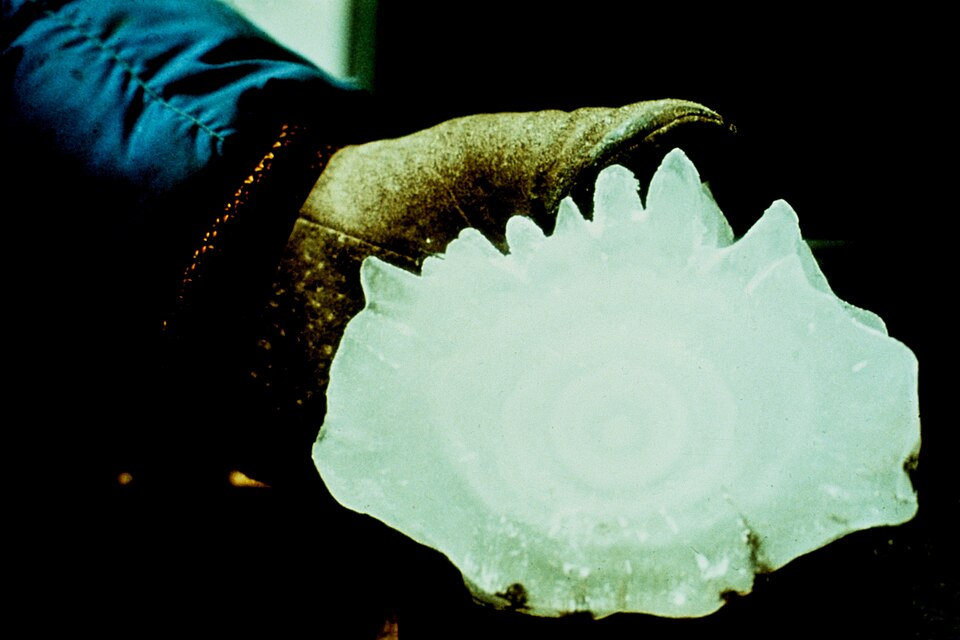
\includegraphics[width=0.5\linewidth]{images/book1/g4-hailstone.jpg}

{\small حبة \omterm{def:g4:clouds-rain-snow:precipitation}{برد} كبيرة جدًا في يد مكسوة بقفاز. الحلقات تبين طبقات الجليد التي
جمعتها في داخل \omterm{def:g4:clouds-rain-snow:cloud}{سحابة} العاصفة. الصورة: مكتبة صور NOAA
(ملك عام).}
% ledger: noaa:photos-g4
\end{omfigure}

\section{نقيس الطقس}

لكي نقول كم أمطرت، أو كم كان الجو دافئًا، أو من أين هبت الريح، لا تكفي
الكلمات: نحتاج إلى أجهزة، وإلى أعداد.

\begin{definition}[مقياس المطر]\label{def:g4:clouds-rain-snow:rain-gauge}
\emph{مقياس المطر}\index{مقياس المطر} وعاء يجمع \omterm{def:g4:clouds-rain-snow:precipitation}{المطر} الساقط على فتحته.
ويُقاس عمق الماء الذي يجمعه بالمليمتر: «5 مليمترات من \omterm{def:g4:clouds-rain-snow:precipitation}{المطر}» معناها أن
\omterm{def:g4:clouds-rain-snow:precipitation}{المطر} كان سيصنع طبقة من الماء عمقها 5 مليمترات على أرض مستوية، لو لم يجرِ
شيء منه ولم يتسرب في الأرض.
\end{definition}

\begin{remark}[مليمتر المطر ماء كثير]\label{rem:g4:clouds-rain-snow:litre}
يبدو مليمتر \omterm{def:g4:clouds-rain-snow:precipitation}{المطر} ضئيلًا في المقياس. لكنه على مربع من الأرض طوله متر وعرضه
متر يساوي لترًا واحدًا من الماء: قارورة كبيرة. وعلى ساحة مدرسة مساحتها ألف
متر مربع، يأتي \omterm{def:g4:clouds-rain-snow:precipitation}{مطر} 10 مليمترات بعشرة آلاف لتر: ما يكفي لملء ألف دلو سعة
كل منها 10 لترات.
\end{remark}

\begin{omfigure}
\begin{tikzpicture}[font=\small]
  % funnel
  \draw[black!70, line width=0.8pt] (-1.2,6.6) -- (-0.35,5.8) -- (-0.35,5.4);
  \draw[black!70, line width=0.8pt] (1.2,6.6) -- (0.35,5.8) -- (0.35,5.4);
  \draw[black!70, line width=0.8pt] (-1.2,6.6) -- (1.2,6.6);
  % tube
  \fill[blue!25] (-0.45,0) rectangle (0.45,2.4);
  \draw[black!70, line width=0.8pt] (-0.45,5.4) -- (-0.45,0) -- (0.45,0) -- (0.45,5.4);
  \foreach \m in {0,1,...,50} {
    \pgfmathsetmacro{\yy}{\m*0.1}
    \draw[black!60] (0.45,\yy) -- ++(-0.12,0);
  }
  \foreach \m in {0,5,10,...,50} {
    \pgfmathsetmacro{\yy}{\m*0.1}
    \draw[black!80] (0.45,\yy) -- ++(-0.25,0);
    \node[anchor=west, font=\scriptsize] at (0.5,\yy) {\m};
  }
  \node[anchor=west, font=\scriptsize] at (1.0,5.0) {mm};
  % reading line
  \draw[red!70!black, -{Stealth}] (-1.6,2.4) -- (-0.5,2.4);
  \node[anchor=east, align=right, font=\scriptsize] at (-1.65,2.4) {اقرأ\\المستوى هنا};
  \node[anchor=west, font=\scriptsize] at (1.9,2.4) {\foreignlanguage{arabic}{\babelsublr{24\,mm} من المطر $\leftarrow$}};
\end{tikzpicture}

{\small مقياس \omterm{def:g4:clouds-rain-snow:precipitation}{مطر} بسيط: قمع يلتقط \omterm{def:g4:clouds-rain-snow:precipitation}{المطر}، وأنبوب مدرّج بالمليمترات يحفظه.
اقرأ مستوى الماء وعينك على الارتفاع نفسه. هنا سقط 24 مليمترًا منذ أفرغ
المقياس آخر مرة.}
\label{fig:g4:clouds-rain-snow:gauge}
\end{omfigure}


\begin{definition}[دوارة الرياح]\label{def:g4:clouds-rain-snow:wind-vane}
\emph{دوارة الرياح}\index{دوارة الرياح} سهم يدور بحرية على سارية. والريح
تدفع ذيله، فيشير السهم دائمًا إلى الجهة التي تأتي \emph{منها}
الريح.
\end{definition}

\begin{definition}[محطة الأرصاد الجوية]\label{def:g4:clouds-rain-snow:weather-station}
\emph{محطة الأرصاد الجوية}\index{محطة الأرصاد الجوية} مكان يُقاس فيه
\omterm{def:g1:watching-the-weather:weather}{الطقس} كل يوم، بالطريقة نفسها دائمًا، بأجهزة: مقياس حرارة في صندوق أبيض
مهوّى، ومقياس \omterm{def:g4:clouds-rain-snow:precipitation}{مطر} في العراء، ودوارة رياح على
سارية.
\end{definition}

يوضع مقياس الحرارة في الظل، في صندوق أبيض جوانبه شرائح تسمح بمرور الهواء
لكنها تمنع أشعة الشمس \omterm{def:g4:clouds-rain-snow:precipitation}{والمطر}. ومصلحة الأرصاد الجوية في المملكة المتحدة
تضعه على ارتفاع
\SI{1.25}{\metre} فوق الأرض. أما \omterm{def:g4:clouds-rain-snow:rain-gauge}{مقياس المطر}
فيقف في العراء، بعيدًا عن الجدران والأشجار التي قد تحجب عنه \omterm{def:g4:clouds-rain-snow:precipitation}{المطر}،
وفتحته أعلى من الأرض بقليل. \omterm{def:g4:clouds-rain-snow:wind-vane}{ودوارة الرياح} تقف عالية على ساريتها، فوق
العوائق التي قد تحرف الريح.
% ledger: mo:screen-height, mo:raingauge

\begin{omfigure}
\begin{tikzpicture}[font=\small, x=1cm, y=1cm]
  % grass
  \fill[green!40!black!45] (-0.5,0) rectangle (11,-0.25);
  \foreach \x in {-0.3,0.1,...,10.8} \draw[green!45!black] (\x,0) -- ++(0.06,0.14);
  % screen on legs
  \draw[black!70, line width=1pt] (0.8,0) -- (0.8,1.25) (2.2,0) -- (2.2,1.25);
  \fill[white, draw=black!70] (0.6,1.25) rectangle (2.4,2.4);
  \foreach \y in {1.4,1.55,...,2.25} \draw[black!40] (0.7,\y) -- (2.3,\y-0.08);
  \fill[white, draw=black!70] (0.45,2.4) -- (1.5,2.75) -- (2.55,2.4) -- cycle;
  \draw[black!60, <->] (2.8,0) -- node[right, font=\scriptsize, align=left] {نحو\\\babelsublr{1.25\,m}} (2.8,1.25);
  \node[align=center, font=\scriptsize] at (1.5,3.25) {مقياس حرارة في\\صندوق أبيض بشرائح};
  % rain gauge
  \fill[black!15, draw=black!70] (5.4,0) rectangle (5.9,0.4);
  \draw[black!70] (5.3,0.55) -- (5.4,0.4) (6.0,0.55) -- (5.9,0.4);
  \node[align=center, font=\scriptsize] at (5.65,1.2) {مقياس مطر\\في العراء};
  % tree far away
  \fill[brown!60!black] (7.3,0) rectangle (7.5,1.3);
  \fill[green!50!black!70] (7.4,2.1) circle (0.85);
  % wind vane on a mast
  \draw[black!70, line width=1pt] (9.8,0) -- (9.8,4.2);
  \draw[black!80, line width=1.4pt, -{Latex[length=3mm]}] (10.6,4.4) -- (9.0,4.4);
  \fill[black!80] (10.6,4.4) -- (10.9,4.65) -- (10.9,4.15) -- cycle;
  \node[align=center, font=\scriptsize] at (9.8,5.05) {دوارة رياح على سارية عالية};
  \node[anchor=west, font=\scriptsize, align=left] at (10.1,3.4) {تشير إلى حيث\\تأتي الريح};
\end{tikzpicture}

{\small \omterm{def:g4:clouds-rain-snow:weather-station}{محطة أرصاد} صغيرة. مقياس الحرارة في الظل، في صندوق أبيض جوانبه
شرائح، على ارتفاع نحو 1.25 متر فوق العشب؛ \omterm{def:g4:clouds-rain-snow:rain-gauge}{ومقياس المطر} في العراء،
بعيدًا عن الشجرة؛ \omterm{def:g4:clouds-rain-snow:wind-vane}{ودوارة الرياح} عالية فوق
العوائق.}
\label{fig:g4:clouds-rain-snow:station}
% ledger: mo:screen-height
\end{omfigure}

\begin{inthefield}[محطة أرصاد في ساحة المدرسة]
مدارس كثيرة تحتفظ \omterm{def:g4:clouds-rain-snow:weather-station}{بمحطة أرصاد} صغيرة في ركن من الساحة. وكل صباح في الوقت
نفسه، يقرأ تلميذان مقياس الحرارة، ويقرآن \omterm{def:g4:clouds-rain-snow:rain-gauge}{مقياس المطر} ويفرغانه، ويسجلان
الجهة التي تشير إليها \omterm{def:g4:clouds-rain-snow:wind-vane}{دوارة الرياح}. ومع مرور الأسابيع يبني الفصل سجلًا
لطقسه الخاص.
\end{inthefield}

\begin{omfigure}
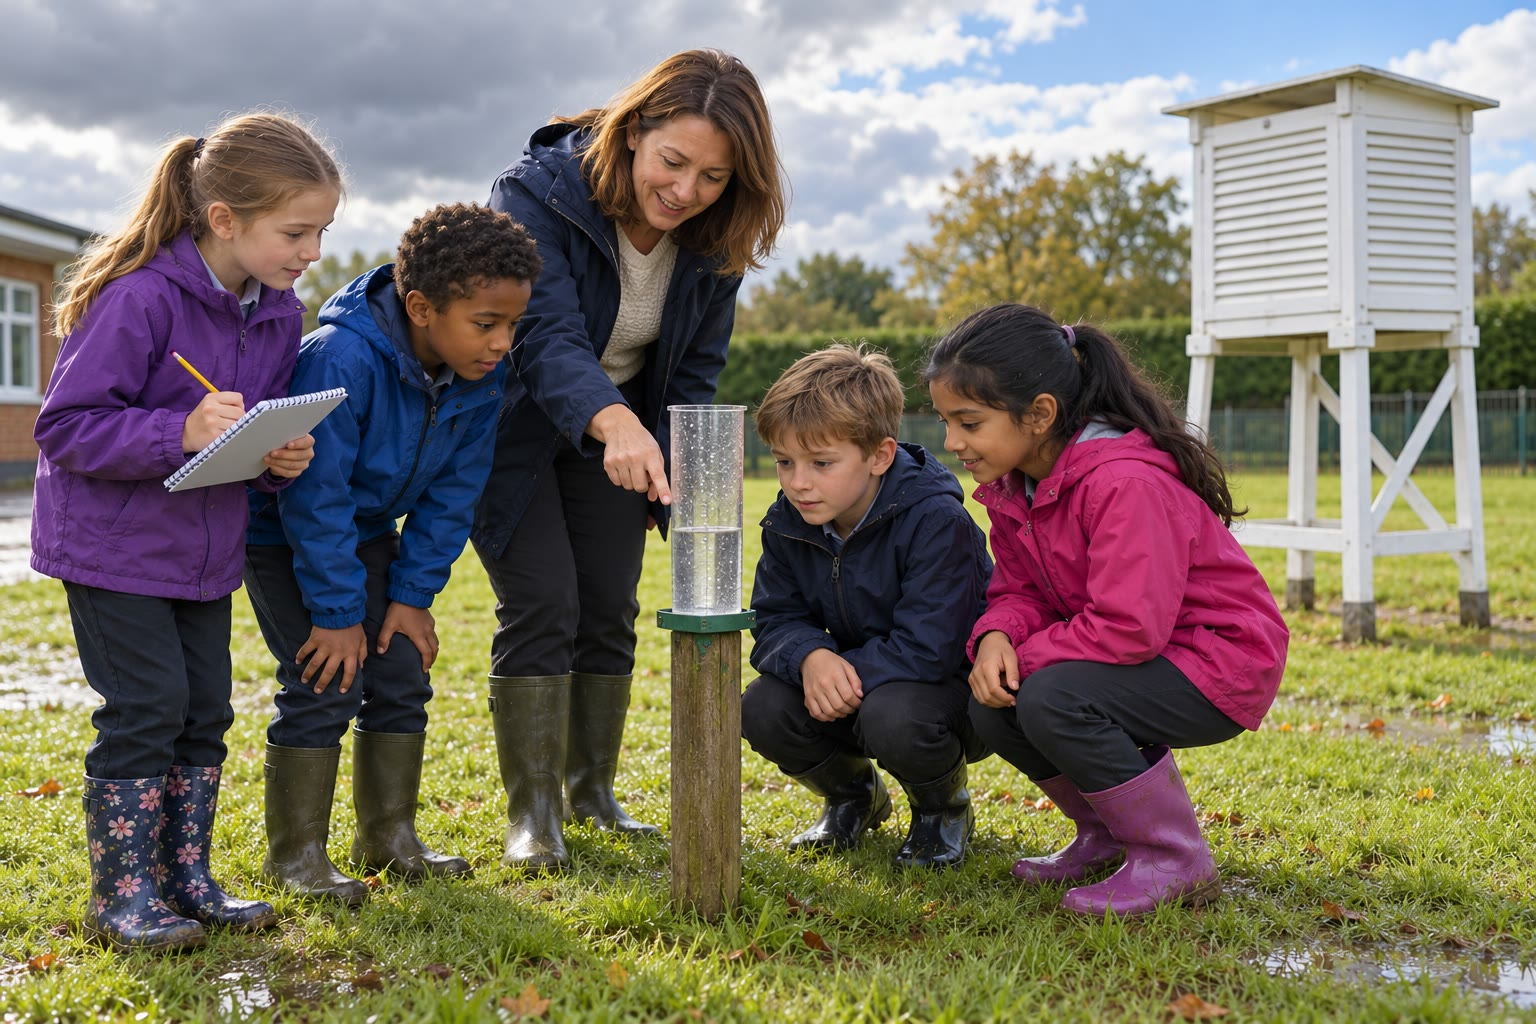
\includegraphics[width=0.55\linewidth]{images/book1/ai/g4-rain-gauge-class.jpg}

{\small تلاميذ يقرؤون \omterm{def:g4:clouds-rain-snow:rain-gauge}{مقياس المطر} في ساحة المدرسة.}
\end{omfigure}

\begin{method}[رسم مخطط أعمدة للمطر]\label{met:g4:clouds-rain-snow:bar-chart}
لرسم \omterm{def:g4:clouds-rain-snow:precipitation}{مطر} أسبوع:
\begin{enumerate}
  \item ارسم خطًا أفقيًا واكتب الأيام تحته، على مسافات متساوية؛
  \item ارسم خطًا رأسيًا على اليسار ودرّجه بالمليمترات، بخطوات
        متساوية (مثلًا كل مليمترين)؛
  \item فوق كل يوم، ارسم عمودًا ارتفاعه بقدر \omterm{def:g4:clouds-rain-snow:precipitation}{مطر} ذلك اليوم؛ واليوم
        الذي لا \omterm{def:g4:clouds-rain-snow:precipitation}{مطر} فيه لا عمود له أبدًا؛
  \item أعطِ المخطط عنوانًا واكتب الوحدة، mm، على الخط
        الرأسي.
\end{enumerate}
\end{method}

\begin{example}[أسبوع من المطر في المدرسة]\label{ex:g4:clouds-rain-snow:week}
قرأ الفصل \omterm{def:g4:clouds-rain-snow:rain-gauge}{مقياس المطر} كل صباح مدة أسبوع فوجد: الاثنين 0، والثلاثاء 4،
والأربعاء 12، والخميس 7، والجمعة 0، والسبت 2، والأحد 5
مليمترات. فأكثر الأيام مطرًا الأربعاء. ولم تمطر يوم الاثنين ولا يوم
الجمعة. وفي الأسبوع كله سقط $0 + 4 + 12 + 7 + 0 + 2 + 5 = 30$
مليمترًا. والأربعاء وحده جاء باثني عشر مليمترًا من الثلاثين، أي
$\frac{12}{30} = \frac{2}{5}$ من \omterm{def:g4:clouds-rain-snow:precipitation}{مطر} الأسبوع.
\end{example}

\begin{omfigure}
\begin{tikzpicture}
\begin{axis}[ybar, bar width=14pt, width=0.8\linewidth, height=5.4cm,
    ymin=0, ymax=14, ytick={0,2,...,14}, ylabel={\foreignlanguage{arabic}{المطر \babelsublr{(mm)}}},
    symbolic x coords={Mon,Tue,Wed,Thu,Fri,Sat,Sun}, xtick=data, xticklabels={الاثنين,الثلاثاء,الأربعاء,الخميس,الجمعة,السبت,الأحد},
    axis x line*=bottom, axis y line*=left, ymajorgrids, grid style={gray!25},
    nodes near coords, nodes near coords style={font=\scriptsize},
    every axis label/.append style={font=\small}, tick label style={font=\small},
    title={المطر في المدرسة خلال أسبوع}, title style={font=\small}]
  \addplot[fill=omWxRain!70, draw=omWxRain!60!black] coordinates
    {(Mon,0) (Tue,4) (Wed,12) (Thu,7) (Fri,0) (Sat,2) (Sun,5)};
\end{axis}
\end{tikzpicture}

{\small أسبوع \cref{ex:g4:clouds-rain-snow:week} في مخطط أعمدة.}
\label{fig:g4:clouds-rain-snow:bars}
\end{omfigure}

\section{تمارين}

\begin{exercise}[$\star$]\label{exo:g4:clouds-rain-snow:1}
مم تتكون \omterm{def:g4:clouds-rain-snow:cloud}{السحابة}؟ وما \omterm{def:g4:clouds-rain-snow:cloud}{الضباب}؟
\end{exercise}

\begin{exercise}[$\star$]\label{exo:g4:clouds-rain-snow:2}
سمِّ \omterm{def:g4:clouds-rain-snow:cloud}{السحابة}: (أ) غطاء رمادي مسطح يحجب السماء كلها؛ (ب) خيوط بيضاء رقيقة
عالية جدًا في سماء زرقاء؛ (ج) أكوام بيضاء قواعدها مسطحة، كأنها
قطن؛ (د) برج داكن ضخم قمته مسطحة، يأتي بالرعد.
\end{exercise}

\begin{exercise}[$\star$]\label{exo:g4:clouds-rain-snow:3}
\omterm{def:g4:clouds-rain-snow:precipitation}{مطر} أم \omterm{def:g4:clouds-rain-snow:precipitation}{ثلج} أم \omterm{def:g4:clouds-rain-snow:precipitation}{برد}؟ (أ) كرات من الجليد تسقط من \omterm{def:g4:clouds-rain-snow:cloud}{سحابة} عاصفة؛ (ب) قطرات
من الماء السائل؛ (ج) ندف مكونة من بلورات الجليد.
\end{exercise}

\begin{exercise}[$\star$]\label{exo:g4:clouds-rain-snow:4}
أي جهاز يقيس: (أ) \omterm{def:g4:clouds-rain-snow:precipitation}{المطر}؛ (ب) درجة الحرارة؛ (ج) الجهة التي تأتي منها
الريح؟
\end{exercise}

\begin{exercise}[$\star$]\label{exo:g4:clouds-rain-snow:5}
في \omterm{def:g4:clouds-rain-snow:rain-gauge}{مقياس المطر} المرسوم في الصفحة~\pageref{fig:g4:clouds-rain-snow:gauge}، يصل الماء
الآن إلى العلامة 17. كم مليمترًا من \omterm{def:g4:clouds-rain-snow:precipitation}{المطر} سقط؟ وكم مليمترًا
آخر يوصله إلى 20؟
\end{exercise}

\begin{exercise}[$\star$]\label{exo:g4:clouds-rain-snow:6}
انظر إلى مخطط الأعمدة في الصفحة~\pageref{fig:g4:clouds-rain-snow:bars}. أي يوم
كان الأكثر مطرًا؟ وفي أي الأيام لم تمطر؟ وأي يوم كان فيه 7
مليمترات؟
\end{exercise}

\begin{exercise}[$\star\star$]\label{exo:g4:clouds-rain-snow:7}
في صباح يوم مثلج، تصل ندف \omterm{def:g4:clouds-rain-snow:precipitation}{الثلج} إلى الأرض في القرية الجبلية، أما في
\omterm{def:g1:landscapes-around-us:landform}{الوادي} تحتها فتمطر. اشرح الفرق،
مستعينًا بدرجة حرارة الهواء.
\end{exercise}

\begin{exercise}[$\star\star$]\label{exo:g4:clouds-rain-snow:8}
في أسبوع آخر وجد الفصل: الاثنين 3، والثلاثاء 0، والأربعاء 1، والخميس
9، والجمعة 6، والسبت 0، والأحد 1 مليمترات. ارسم مخطط الأعمدة. كم
مليمترًا سقط في الأسبوع؟ وأي كسر من \omterm{def:g4:clouds-rain-snow:precipitation}{مطر} الأسبوع سقط يوم
الخميس؟
\end{exercise}

\begin{exercise}[$\star\star$]\label{exo:g4:clouds-rain-snow:9}
لماذا يجب أن يقف \omterm{def:g4:clouds-rain-snow:rain-gauge}{مقياس المطر} في العراء، بعيدًا عن الجدران والأشجار؟ ولماذا
يوضع مقياس الحرارة في صندوق أبيض في الظل، لا في الشمس الساطعة؟
\end{exercise}

\begin{exercise}[$\star\star$]\label{exo:g4:clouds-rain-snow:10}
\omterm{def:g4:clouds-rain-snow:wind-vane}{دوارة الرياح} تشير إلى الغرب. من أين تأتي الريح؟ وإلى أين
تذهب؟
\end{exercise}

\begin{exercise}[$\star\star\star$]\label{exo:g4:clouds-rain-snow:11}
على ساحة مساحتها 500 متر مربع، يسقط 8 مليمترات من \omterm{def:g4:clouds-rain-snow:precipitation}{المطر}. مستعينًا
بما في \cref{rem:g4:clouds-rain-snow:litre}، كم لترًا من الماء سقط على
الساحة؟ وإذا كان المرش يتسع 10 لترات: فكم مرشًا يساوي ذلك؟
\end{exercise}
